\documentclass[12pt]{article}

\usepackage[english]{babel}
\usepackage{graphicx}
\usepackage{setspace}
\usepackage{parskip}
\usepackage{indentfirst}

\pagestyle{empty}
\setcounter{secnumdepth}{2}

\topmargin=0cm
\oddsidemargin=0cm
\textheight=22.0cm
\textwidth=16cm
\parindent=1cm
\parskip=0.15cm
\topskip=0truecm
\raggedbottom
\abovedisplayskip=3mm
\belowdisplayskip=3mm
\abovedisplayshortskip=0mm
\belowdisplayshortskip=2mm
\normalbaselineskip=12pt
\normalbaselines

\begin{document}



%%%%%%%%%%%%%%%%%%%%%%%%%%%%%%%%%%%%%%%%%%%%%%%%%%%%%%%%%%%%%%
%                        First page                         
%%%%%%%%%%%%%%%%%%%%%%%%%%%%%%%%%%%%%%%%%%%%%%%%%%%%%%%%%%%%%%


\vspace*{0.5in}
\centerline{\bf\Large Deliverable 2}
\vspace*{0.2in}
\centerline{\bf\Large Project Design Document}

\vspace*{1.7in}
\centerline{\bf\Large C-Labs}
\vspace*{0.2in}
\centerline{
\begin{tabular}{c c}
      Ashwath George & 9733469\\
      Nicholas Gignac & 9128964\\
      Robert Jakubowicz & 6045707\\
      Caroline Labbe & 6320945\\
      Brian Lam & 1696785\\\\
\end{tabular}}

\vspace*{1.2in}
\centerline{\bf\Large For the course:}
\centerline{\bf\Large COMP354}
\centerline{\bf\Large Introduction to Software Engineering}

\vspace*{0.8in}
\centerline{Presented to:}
\centerline{Sutharsan Sivagnanam}
\centerline{July 24, 2013}

\clearpage

\setcounter{secnumdepth}{3}
\tableofcontents
\clearpage
\listoffigures
\listoftables

\clearpage

\pagestyle{plain}
\doublespacing


%%%%%%%%%%%%%%%%%%%%%%%%%%%%%%%%%%%%%%%%%%%%%%%%%%%%%%%%%%%%%%
%                       Introduction                        
%%%%%%%%%%%%%%%%%%%%%%%%%%%%%%%%%%%%%%%%%%%%%%%%%%%%%%%%%%%%%%


\section{Introduction}
\par
The C-Ker program, from C-Labs, is a Vessel Monitoring System, delivered during the course of COMP 354, where the teacher will be referred to as the ‘customer’. For this second delivery, this document brings up more accurate information about the Architectural Design of the software in more details, as well as provides Dynamic Design scenarios. We will also review the Cost Estimation originally done in Delivery 1, using the data and experience acquired during this delivery as well as the previous.



%%%%%%%%%%%%%%%%%%%%%%%%%%%%%%%%%%%%%%%%%%%%%%%%%%%%%%%%%%%%%%
%                       Part 2                       
%%%%%%%%%%%%%%%%%%%%%%%%%%%%%%%%%%%%%%%%%%%%%%%%%%%%%%%%%%%%%%



\section{Architectural Design}
\par
In our project, we decided to use the MVP (Model-View-Presenter) architecture pattern instead of MVC. Both are very similar except for the workflow, and the Presenter and Controller which have different roles. MVP was selected over MVC because it reflects our workflow more accurately. In MVP, the user interacts with the View, which then sends the commands to the Presenter who returns the data for the View to display after having interacted with the Model. In MVC, the user interacts with the Controller, which depending on the user’s action, will interact with the Model and send the data to the View. Additional, if there is an update on the Model, the view can be notified. In MVP, the View never communicates with the Model, everything is done through the Presenter.
\par
As seen in Figure~\ref{fig:HighLevelArchitecture} below, the system contains four subsystems: GUI, Authentication, Simulation and Parsing. The GUI's purpose it to display Widgets and let the user interact with the system. Authentication is used to validate the credentials of a user and only grants access to authorized users. Simulation performs the calculations on the vessels. Finally, Parsing is used to read scenario files.

\begin{figure}[h!]
    \centering
    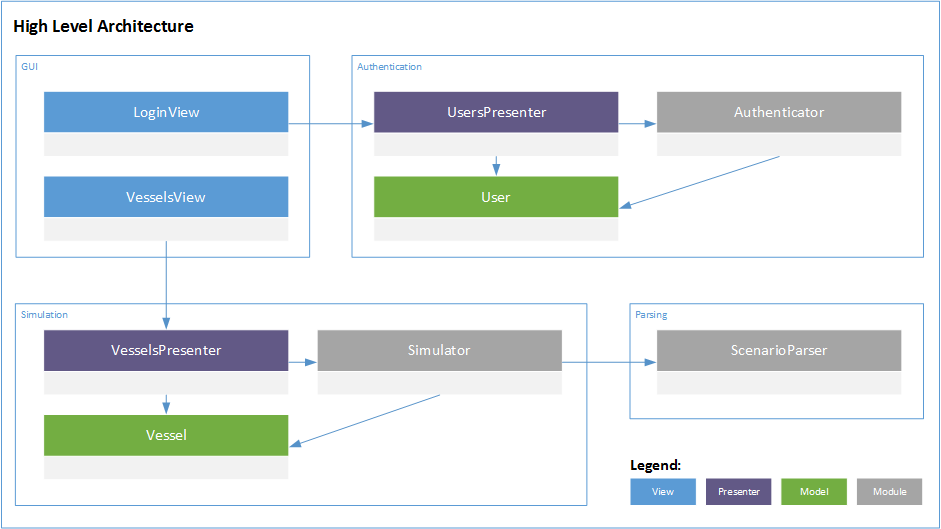
\includegraphics[scale=0.63]{4+1HighLevel}
    \caption{High Level Architecture}
    \label{fig:HighLevelArchitecture}
\end{figure}


\subsection{Architecture Diagram}
\par
The structure of the system is depicted using a 4+1 architectural view.

\subsubsection{Logical View}
\par
Our system provides the user with four main functionalities: authentication, vessel viewing, 
vessel movement and alarms, as well as scenario file parsing. These functionalities are provided
using components illustrated in the class diagram in Figure~\ref{fig:UMLClassDiagram}.
\clearpage

\begin{figure}[h!]
    \centering
    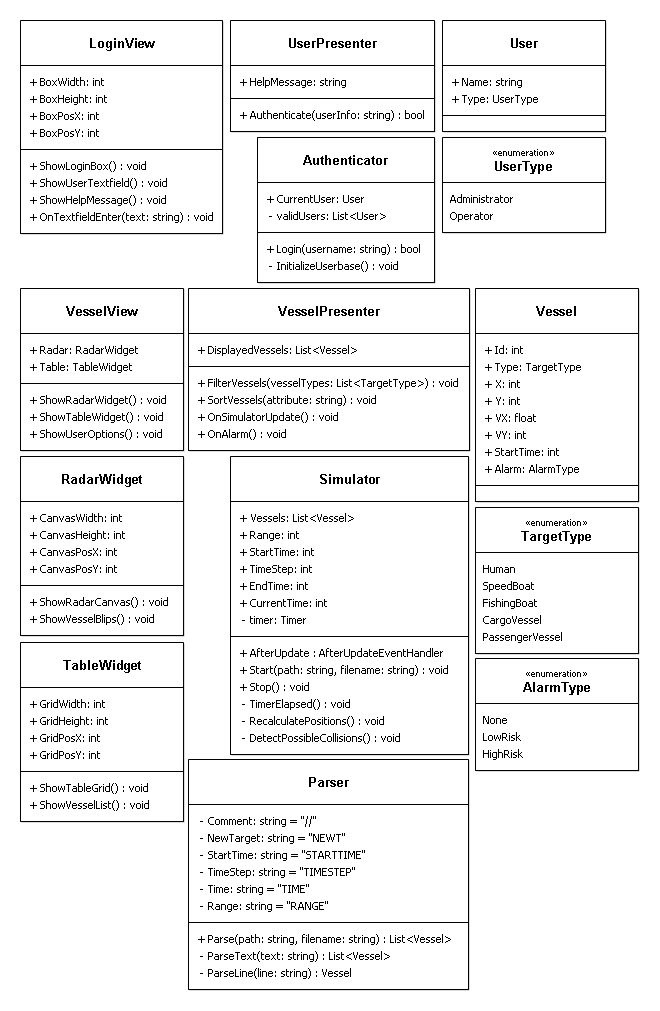
\includegraphics[scale=0.75]{3_ClassDiagram}
    \caption{System Class diagram}
    \label{fig:UMLClassDiagram}
\end{figure}

\par
Authentication allows users to login and access the system. As shown in Figure~\ref{fig:AuthenticateSequenceDiagram}, the Authenticate() function is called with the username. If the specific username is allowed access, the Authenticate() returns true and false otherwise. Different user types have different priviledges when viewing the vessels.

\begin{figure}[h!]
    \centering
    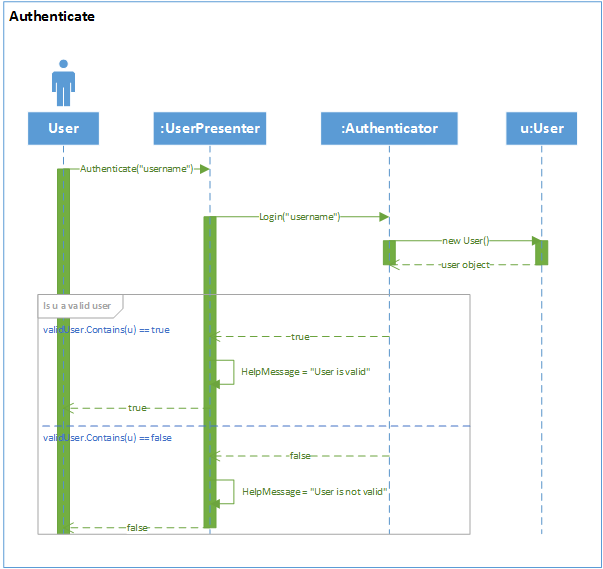
\includegraphics[scale=1]{2_1_authenticate}
    \caption{Authenticate Sequence Diagram}
    \label{fig:AuthenticateSequenceDiagram}
\end{figure}

\par
Vessel viewing allows users to observe vessels in both table list form and radar map form.
Furthermore, users can filter and sort vessels that are displayed. As shown in Figure~\ref{fig:FilteringSequenceDiagram}, filtering is performed by the VesselsPresenter by calling the function GetVessels() and passing the type to filter on. It returns a filtered list of vessels which is then used to update the table and radar.

\begin{figure}[h!]
    \centering
    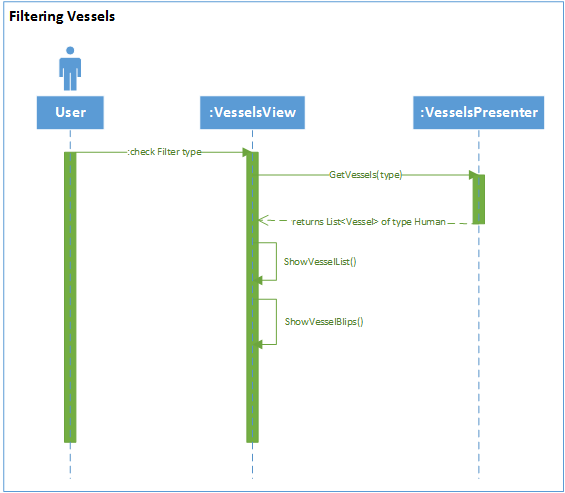
\includegraphics[scale=1]{2_1_filtering}
    \caption{Filtering Sequence Diagram}
    \label{fig:FilteringSequenceDiagram}
\end{figure}

As shown in Figure~\ref{fig:SortingSequenceDiagram}, sorting is performed by the VesselsPresenter by calling the function SortVessels() and passing the attribute to sort on. It returns a sorted list of vessels which is then used by VesselView.
\clearpage
\begin{figure}[h!]
    \centering
    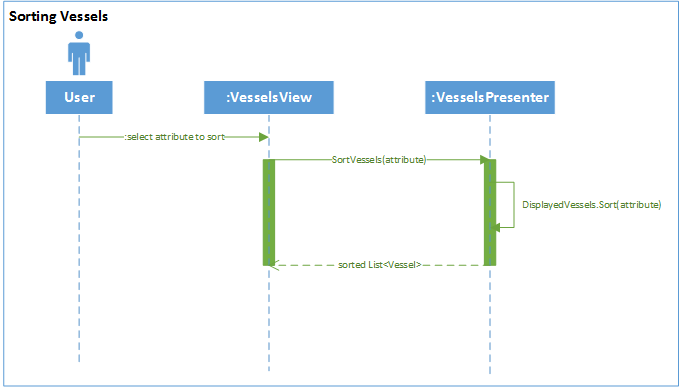
\includegraphics[scale=1]{2_1_sorting}
    \caption{Sorting Sequence Diagram}
    \label{fig:SortingSequenceDiagram}
\end{figure}

\par
Vessel movement and alarms allows users to receive dynamic updates of the vessels current statuses. As illustrated in Figure~\ref{fig:RecalculatePositionsSequenceDiagram}, the Simulator loops until the EndTime is reached. At each iteration, it recalculates the position and notifies the VesselPresenter that the positions have been updated by raising an event.
\clearpage

\begin{figure}[h!]
    \centering
    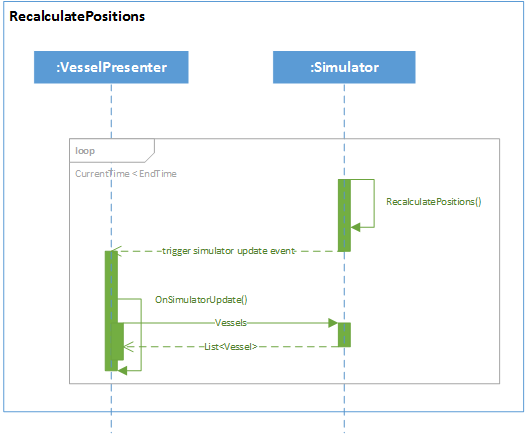
\includegraphics[scale=1]{2_1_recalculate_positions}
    \caption{Recalculate Positions Sequence Diagram}
    \label{fig:RecalculatePositionsSequenceDiagram}
\end{figure}

\par
Parsing allows scenario files to be read in order to load simulation properties and vessel initial data. As seen in Figure~\ref{fig:ParseSequenceDiagram}, the function Parse() is call and passed the path and the filename of the scenario file. First the text is parsed, and then each line of the text. A list of vessels is returned to the Simulator.

\begin{figure}[h!]
    \centering
    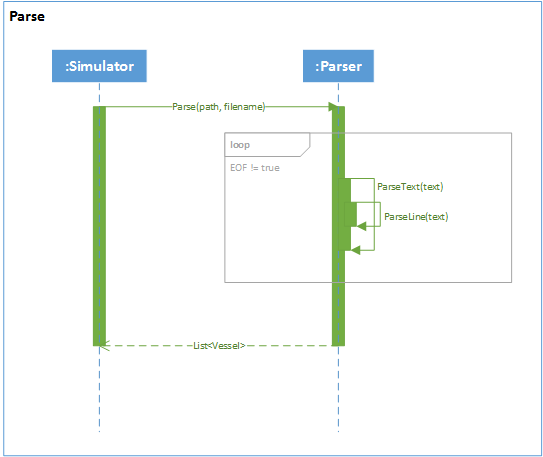
\includegraphics[scale=1]{2_1_parse}
    \caption{Parse Sequence Diagram}
    \label{fig:ParseSequenceDiagram}
\end{figure}

\clearpage


\subsubsection{Development View}
\par
The static organization of the C-Ker Vessel Monitoring System in its development environment is demonstrated through the use of a Component Diagram. As shown in Figure~\ref{fig:UMLComponentDiagram}, the decomposition of the C-Ker code base into four distinct code components allows for a clearer view of their implementations, including the interdependencies between the modules contained within. This serves as a basis for requirement allocation and the allocation of work to the programmers, while also facilitating a comprehensive estimation the cost evaluation and planning stages of the project.

\begin{figure}[h!]
    \centering
    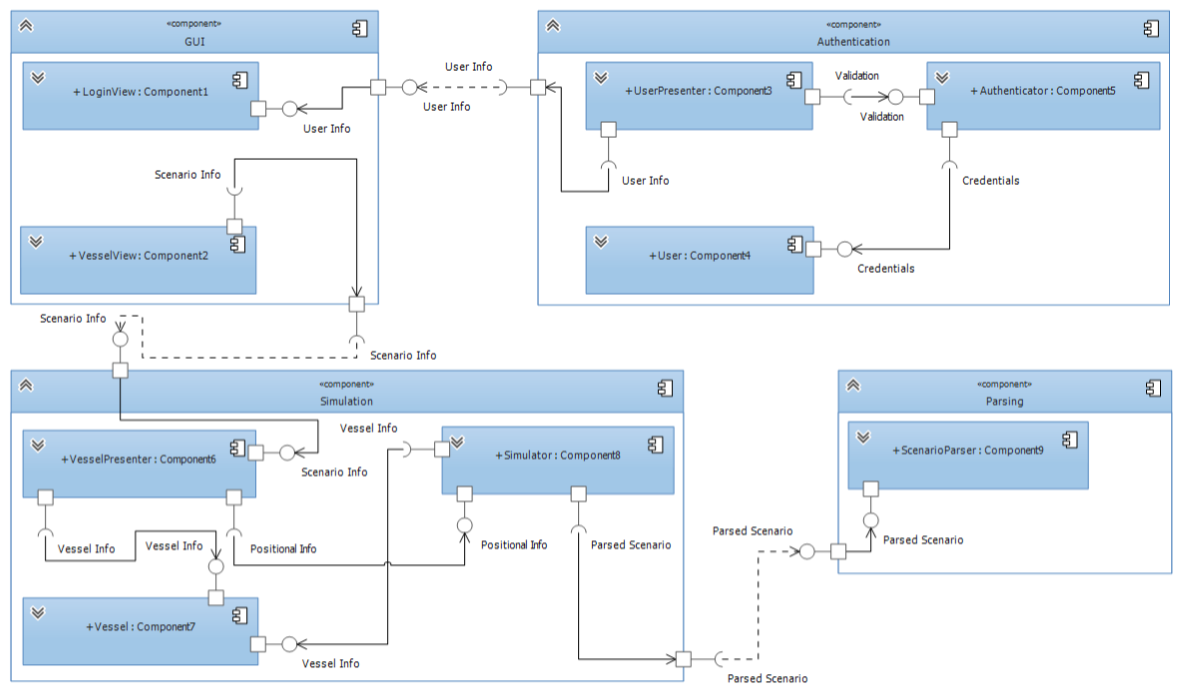
\includegraphics[scale=0.5]{section_2_component_diagram}
    \caption{Component Diagram}
    \label{fig:UMLComponentDiagram}
\end{figure}
\clearpage


\subsubsection{Process View}
\par
The concurrency and synchronization aspects of the design of the C-Ker System can be best characterized through an Activity Diagram. Figure~\ref{fig:UMLActivityDiagram} depicts the runtime behaviour of the system as a whole, highlighting the mapping of logical components to processes. Figure~\ref{fig:AlarmActivityDiagram}, on the other hand, focuses on the manner in which the system handles the process of triggering alarms by modelling the concurrent behaviour of the Simulation subsystem.

\begin{figure}[h!]
    \centering
    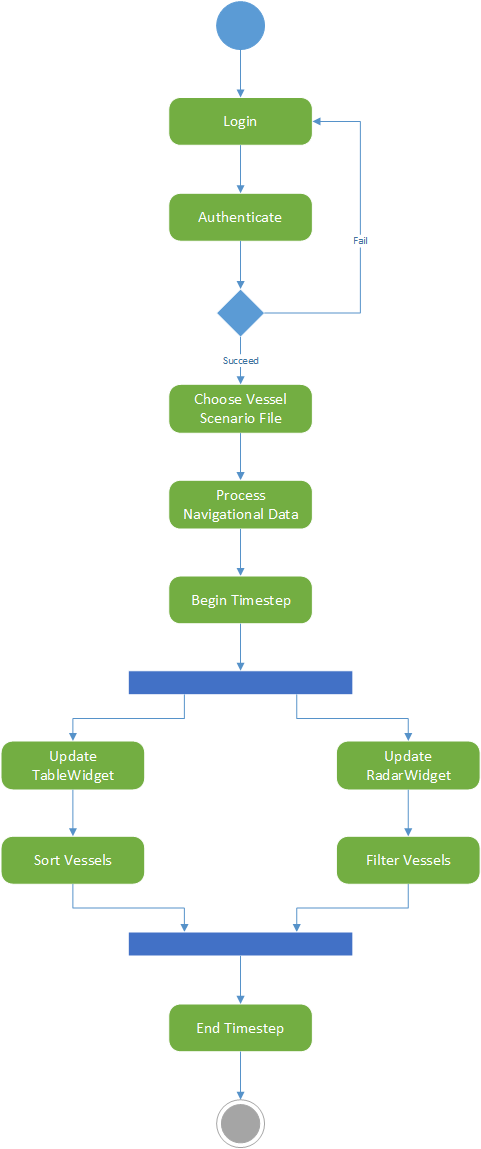
\includegraphics[scale=0.65]{section_2_activity_diagram}
    \caption{Main Activity diagram}
    \label{fig:UMLActivityDiagram}
\end{figure}
\clearpage
\begin{figure}[h!]
    \centering
    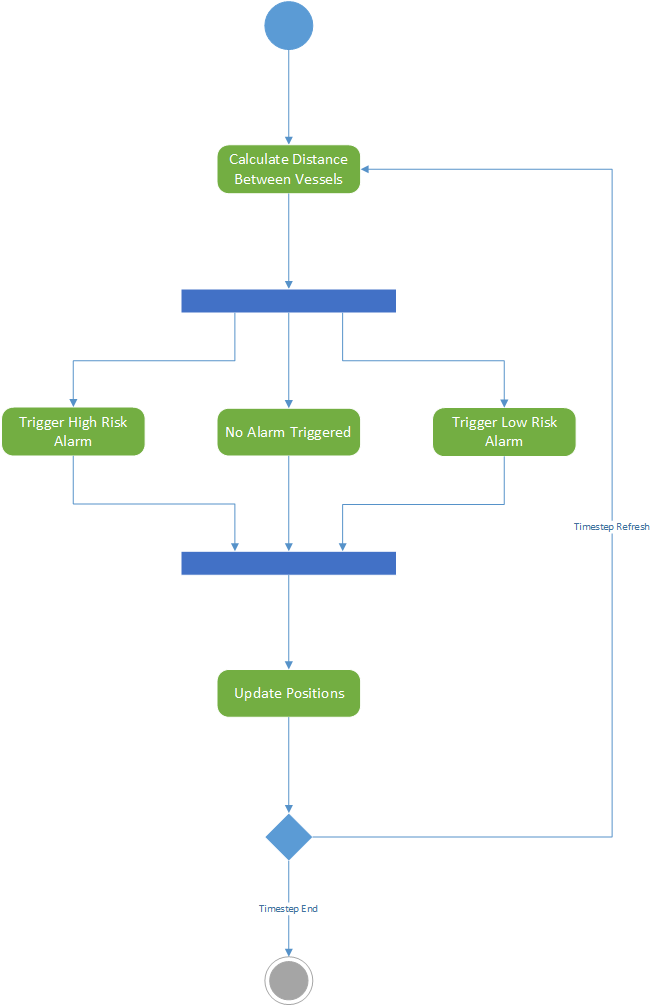
\includegraphics[scale=0.75]{alarm_activity_diagram}
    \caption{Alarm Activity Diagram}
    \label{fig:AlarmActivityDiagram}
\end{figure}
\clearpage


\subsubsection{Physical View}
This view does not apply to our project.


%%%%%%%%%%%%%%%%%%%%%%%%%%%%%%%%%%%%%%%%%%%%%%%%%%%%%%%%%%%%%%
%                         Scenarios                          %
%%%%%%%%%%%%%%%%%%%%%%%%%%%%%%%%%%%%%%%%%%%%%%%%%%%%%%%%%%%%%%

\subsubsection{Scenarios}

The architecture is further illustrated using a set of use cases as shown in Figure~\ref{fig:UseCaseDiagram}.
\begin{figure}[h!]
    \centering
    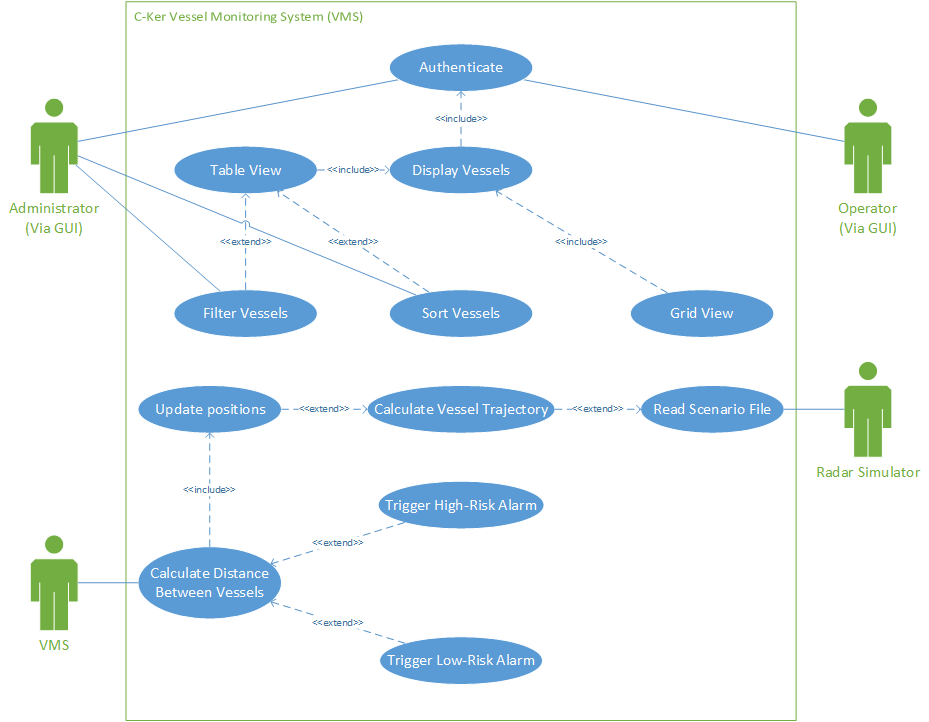
\includegraphics[scale=0.65]{UCD}
    \caption{Use Case diagram}
    \label{fig:UseCaseDiagram}
\end{figure}
\clearpage

\vspace*{0.2in}
\centerline{\textsc{Scenarios}}
\vspace*{0.2in}

\begin{table}[ht]
\centering
   \begin{tabular}{|l|l|}
        \hline
        {\large Name} & {\large Listing Vessels in a Table} \\
        \hline\hline
        Actors & Any user, TableView, Presenter\\
        \hline
        Goals & Allow users to view vessel information listed in a         table\\
        \hline
        Pre-conditions & Vessel information must be loaded and updated correctly\\
        \hline
        Summary & Information about each vessel is displayed in a table format\\
        \hline
        Related Use Cases & Updating Vessel Positions\\
        \hline
        Steps & - \ The TableView retrieves vessel information from the Presenter\\
         & - \ The application displays vessel information in a table on\\
          & \ \ \ screen\\
          & - \ The user views vessel information as desired\\
        \hline
        Post-conditions & The vessel information are listed in a table on screen\\
        \hline
        Difficulty & Low\\
        \hline
        Importance & High\\
        \hline
    \end{tabular}
\caption{Listing Vessels in a Table}
\end{table}


\begin{table}[ht]
\centering
   \begin{tabular}{|l|l|}
        \hline
        {\large Name} & {\large Filtering Vessels by Type} \\
        \hline\hline
        Actors & User with admin privileges\\
        \hline
        Goals & Allow users to view or hide certain vessel types only\\
        \hline
        Pre-conditions & - \ Vessel information must be loaded and listed correctly\\
         & - \ User must be authenticated as an administrator\\
        \hline
        Summary & The displayed vessel information can be filtered by vessel type\\
        \hline
        Related Use Cases & Listing Vessels in a Table\\
        \hline
        Steps & - \ The user selects vessel types to be filtered through the\\
         & \ \ \ interface\\
         & - \ The application shows only the wanted vessel types on screen\\
          & - \ The user views vessel information as desired\\
        \hline
        Post-conditions & The vessels displayed match the filtering options\\
        \hline
        Difficulty & Medium\\
        \hline
        Importance & High\\
        \hline
    \end{tabular}
\caption{Filtering Vessels by Type}
\end{table}



\begin{table}[ht]
\centering
   \begin{tabular}{|l|l|}
        \hline
        {\large Name} & {\large Sorting Vessels by Data} \\
        \hline\hline
        Actors & User with admin privileges\\
        \hline
        Goals & Allow users to organize and view vessels with more flexibility\\
        \hline
        Pre-conditions & - \ Vessel information must be loaded and listed correctly\\
         & - \ User must be authenticated as an administrator\\
        \hline
        Summary & The displayed vessel information can be sorted according to\\
         & selected data\\
        \hline
        Related Use Cases & Listing Vessels in a Table\\
        \hline
        Steps & - \ The user selects a data type through the application interface\\
         & - \ The application sorts the listing according to the selected data\\
          & - \ The user views vessel information as desired\\
        \hline
        Post-conditions & The vessels displayed match the filtering options\\
        \hline
        Difficulty & Medium\\
        \hline
        Importance & High\\
        \hline
    \end{tabular}
\caption{Sorting Vessels by Data}
\end{table}



\begin{table}[ht]
\centering
   \begin{tabular}{|l|l|}
        \hline
        {\large Name} & {\large Displaying Vessels on Radar} \\
        \hline\hline
        Actors & Any user, RadarView, Presenter\\
        \hline
        Goals & Give users a top-down visualization of the simulation in 2D\\ 
         & space\\
        \hline
        Pre-conditions & Vessel information must be updated continuously and correctly\\
        \hline
        Summary & Vessels are represented graphically through blips on a radar\\ 
         & display\\
        \hline
        Related Use Cases & Updating Vessel Positions\\
        \hline
        Steps & - \ The RadarView retrieves vessel information from the\\ 
         & \ \ \ Presenter\\
         & - \ The application draws the radar, with blips representing vessel\\ 
         & \ \ \ positions\\
         & - \ The radar is redrawn at regular intervals to reflect updates in\\ 
         & \ \ \ simulation\\
         & - \ The user views the map and vessels as desiredn\\
        \hline
        Post-conditions & The vessel information are listed in a table on screen\\
        \hline
        Difficulty & Medium\\
        \hline
        Importance & High\\
        \hline
    \end{tabular}
\caption{Displaying Vessels on Radar}
\end{table}




\begin{table}[ht]
\centering
   \begin{tabular}{|l|l|}
        \hline
        {\large Name} & {\large Loading Vessel Information} \\
        \hline\hline
        Actors & Simulator\\
        \hline
        Goals & Load vessel information into memory from a scenario file\\
        \hline
        Pre-conditions & Scenario file must exist and be formatted correctly\\
        \hline
        Summary & The radar simulator reads information on simulation and vessel\\ 
         & properties\\
        \hline
        Related Use Cases & None\\
        \hline
        Steps & - \ A specific scenario file is provided\\
         & - \ The simulator reads the file, parses the relevant info, and\\ 
         & \ \ \ stores it\\
        \hline
        Post-conditions & All simulation and vessel data are loaded and ready to be\\ 
         & simulated\\
        \hline
        Difficulty & Low\\
        \hline
        Importance & High\\
        \hline
    \end{tabular}
\caption{Loading Vessel Information}
\end{table}





\begin{table}[ht]
\centering
   \begin{tabular}{|l|l|}
        \hline
        {\large Name} & {\large Updating Vessel Positions} \\
        \hline\hline
        Actors & Simulator\\
        \hline
        Goals & Simulate vessel movement at regular intervals\\
        \hline
        Pre-conditions & Vessel information must be loaded correctly\\
        \hline
        Summary & The radar simulator plots vessel trajectories by performing\\
         & the necessary physics calculations using the information\\
         & parsed from the corresponding scenario file.\\
        \hline
        Related Use Cases & Loading Vessel Information\\
        \hline
        Steps & - \ The simulator begins with the initial position of the vessel\\
         & - \ The vessel’s subsequent positions are calculated over time,\\
         & \ \ \ based on its velocity along the coordinate axes\\
        \hline
        Post-conditions & Vessel positions are updated correctly\\
        \hline
        Difficulty & Low\\
        \hline
        Importance & High\\
        \hline
    \end{tabular}
\caption{Updating Vessel Positions}
\end{table}




\begin{table}[ht]
\centering
   \begin{tabular}{|l|l|}
        \hline
        {\large Name} & {\large Triggering Risk Alarms} \\
        \hline\hline
        Actors & Simulator\\
        \hline
        Goals & Trigger alarms to warn users when vessels get too close to\\
         & each other\\
        \hline
        Pre-conditions & Vessel information must be updated continuously and correctly\\
        \hline
        Summary & The radar simulator calculates distances between vessels, and\\
         & triggers specific alarms under certain conditions.\\
        \hline
        Related Use Cases & Updating Vessel Positions\\
        \hline
        Steps & - \ The simulator calculates distances between vessels after every\\
         & \ \ \ update\\
         & - \ If the distance between any two vessels is between 200m and\\
         & \ \ \  50m, the simulator triggers a Low Risk Alarm for those vessels\\
          & - \ If the distance between any two vessels is less than 50m, the\\
         & \ \ \ simulator triggers a High Risk Alarm for those vessels\\
        \hline
        Post-conditions & Alarms are triggered if conditions are met\\
        \hline
        Difficulty & Low\\
        \hline
        Importance & High\\
        \hline
    \end{tabular}
\caption{Triggering Risk Alarms}
\end{table}
\clearpage


%%%%%%%%%%%%%%%%%%%%%%%%%%%%%%%%%%%%%%%%%%%%%%%%%%%%%%%%%%%%%%
%                       Part 2.2                      
%%%%%%%%%%%%%%%%%%%%%%%%%%%%%%%%%%%%%%%%%%%%%%%%%%%%%%%%%%%%%%


\subsection{Subsystem Interfaces Specifications}

The purpose of this Subsystem Interface Specification is to describe the messages and function calls that are exchanged between the various modules of the C-Ker Vessel Monitoring System. It is intended to specify the externally observable behavior of a module’s access routines, including input/output relationships and parameters that could be considered either valid or invalid. 
\par
The Figures in sections 2.2.1 and 2.2.2 provide specifications for interfaces within the GUI subsystem, sections 2.2.3 to 2.2.6 belong to the Authentication subsystem, sections 2.2.7 and 2.2.8 belong to the Simulation subsystem, and finally section 2.2.9 belongs to the Parsing subsystem.
\par
\begin{figure}[h!]
    \centering
    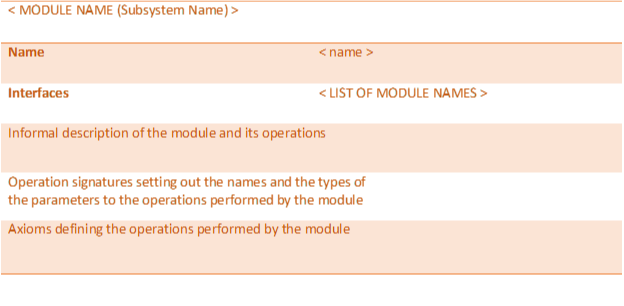
\includegraphics[scale=0.9]{figure_2_2}
    \caption{Subsystem Interface Specification template}
    \label{fig:SubsystemInterfaceSpecificationTemplate}
\end{figure}
The structure of the Subsystem Interface Specification is shown in Figure~\ref{fig:SubsystemInterfaceSpecificationTemplate}. The body of the specification has four components:
\par

1.  \ An introduction that declares the name of the module being specified. The introduction may also include an ‘Interfaces’ declaration, which lists the other subsystems with which the current module interfaces, if any.\par
2.	\ A description, which informally describes the module and the operations (functions or methods/member functions) it performs. This allows for easier interpretation of the formal specification. \par
3.	\ The signature part, which defines the syntax of the interface between the modules. The names of the operations that are defined, the data types of their arguments, parameters and outputs are described in the signature.\par
4.	\ The axioms part, which characterizes the behavior of the operations by defining the valid range of inputs required for the operation to be carried out successfully.
\par

\subsubsection{LoginView Module: GUI Subsystem}
\begin{figure}[h!]
    \centering
    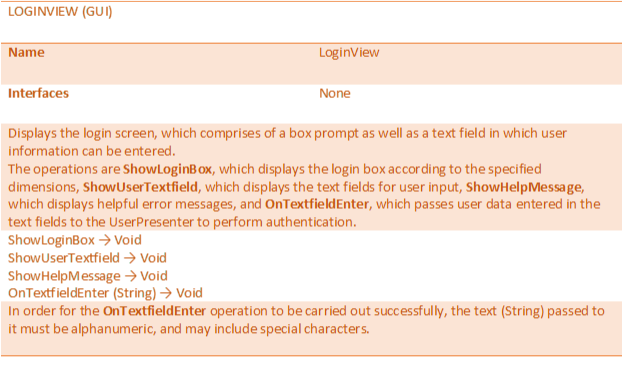
\includegraphics[scale=0.9]{2_2_1_loginview_(gui)}
    \caption{LoginView}
\end{figure}
\clearpage

\subsubsection{VesselView Module: GUI Subsystem}
\begin{figure}[h!]
    \centering
    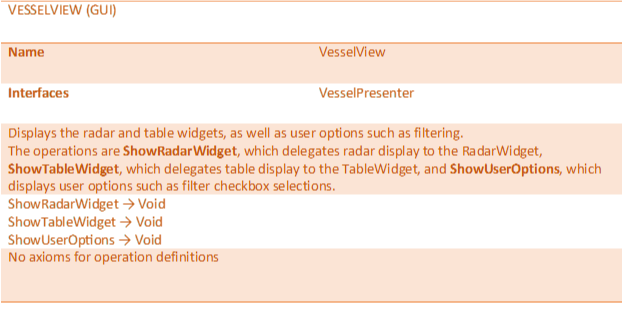
\includegraphics[scale=0.9]{2_2_2_vesselview_(gui)}
    \caption{VesselView}
\end{figure}

\subsubsection{UserPresenter Module: Authentication Subsystem}
\begin{figure}[h!]
    \centering
    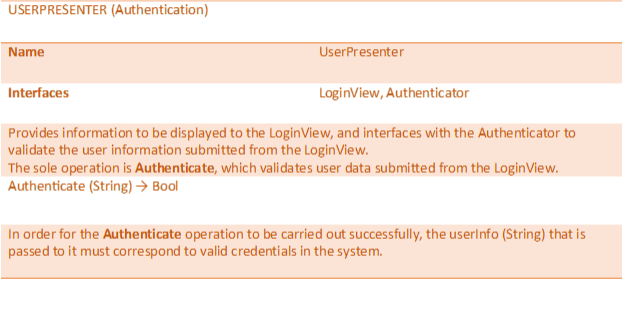
\includegraphics[scale=0.9]{2_2_3_userpresenter_(authentication)}
    \caption{UserPresenter Module}
\end{figure}

\subsubsection{Authenticator Module: Authentication Subsystem}
\begin{figure}[h!]
    \centering
    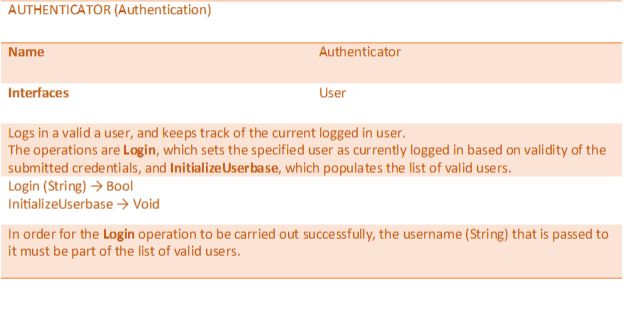
\includegraphics[scale=0.9]{2_2_4_authenticator_(authentication)}
    \caption{Authenticator Module}
\end{figure}

\subsubsection{User Module: Authentication Subsystem}
\begin{figure}[h!]
    \centering
    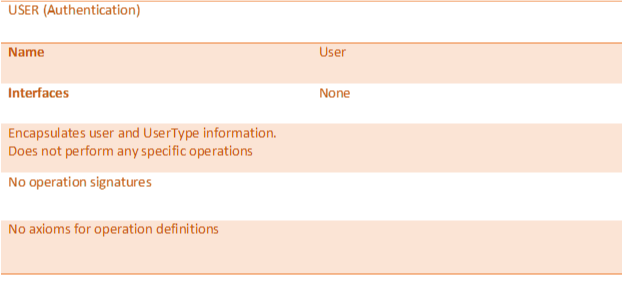
\includegraphics[scale=0.9]{2_2_5_user_(authentication)}
    \caption{User Module}
\end{figure}
\clearpage

\subsubsection{VesselPresenter Module: Simulation Subsystem}
\begin{figure}[h!]
    \centering
    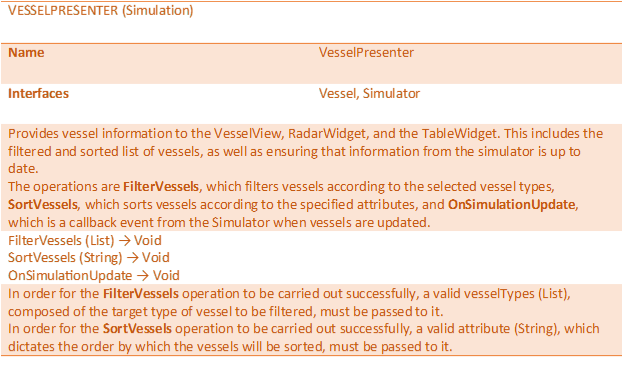
\includegraphics[scale=0.9]{2_2_6_vesselpresenter_(simulation)}
    \caption{VesselPresenter Module}
\end{figure}
\clearpage

\subsubsection{Simulator Module: Simulation Subsystem}
\begin{figure}[h!]
    \centering
    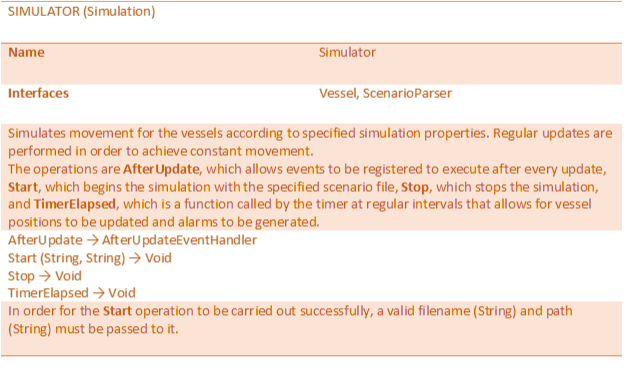
\includegraphics[scale=0.9]{2_2_7_simulator_(simulation)}
    \caption{Simulator Module}
\end{figure}
\clearpage

\subsubsection{Vessel Module: Simulation Subsystem}
\begin{figure}[h!]
    \centering
    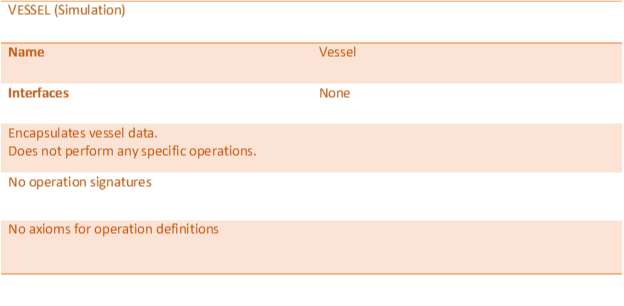
\includegraphics[scale=0.9]{2_2_8_vessel_(simulation)}
    \caption{Vessel Module}
\end{figure}

\subsubsection{ScenarioParser Module: Parsing Subsystem}
\begin{figure}[h!]
    \centering
    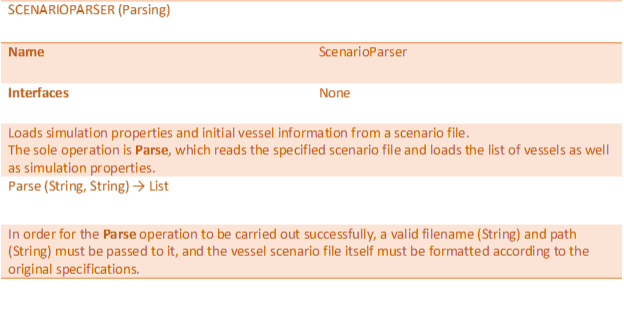
\includegraphics[scale=0.9]{2_2_9_scenarioparser_(parsing)}
    \caption{ScenarioParser Module}
\end{figure}
\clearpage



%%%%%%%%%%%%%%%%%%%%%%%%%%%%%%%%%%%%%%%%%%%%%%%%%%%%%%%%%%%%%%
%                       Part 3                       
%%%%%%%%%%%%%%%%%%%%%%%%%%%%%%%%%%%%%%%%%%%%%%%%%%%%%%%%%%%%%%

\section{Detailed Design}

The system is divided into four subsystems: GUI, Authentication, Simulation, and Parsing. They each handle independent responsibilities which makes the system easier to understand and to maintain.


\subsection{GUI Subsystems}
The GUI subsystem takes care of displaying information on screen; it also provides the user with an interface to use the application.


\subsubsection{Detailed Design Diagram}
This subsystem consists of the LoginView, the VesselView, the RadarWidget, and the TableWidget classes as shown in Figure~\ref{fig:GUISubsystemClassDiagram}. This design allows the GUI elements to be modularized and isolated.
\begin{figure}[h!]
    \centering
    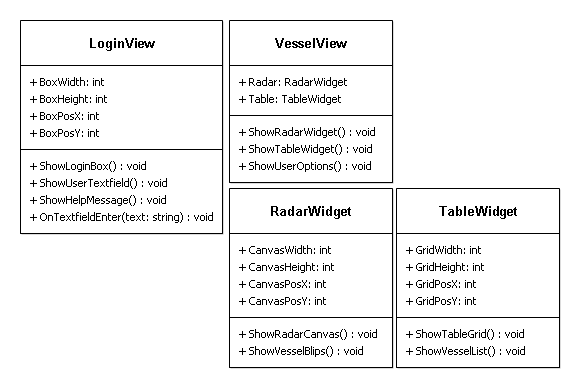
\includegraphics[scale=0.8]{3_1_1_guisubsystem}
    \caption{GUI Subsystem Class diagram}
    \label{fig:GUISubsystemClassDiagram}
\end{figure}


\subsubsection{Unit Descriptions}
\vspace*{0.2in}
\leftline{\textsc{LoginView}}
\vspace*{0.15in}
LoginView’s purpose is to display the login screen; this includes a box prompt as well as a text field in which user information can be entered.

\begin{table}[ht]
\centering
   \begin{tabular}{|l|l|}
        \hline
        {\large Name} & {\large Description} \\
        \hline\hline
        BoxWidth &  \\
        BoxHeight &  Defines the dimensions of the login prompt.\\
        BoxPosX &  \\
        BoxPosY &  \\
        \hline
        ShowLoginBox & Displays the login box according to dimensions.\\
        \hline
        ShowUserTextfield & Displays the text field for the user information to be entered.\\
        \hline
        ShowHelpMessage & Displays any messages which help inform the user; the 
        \\ & messages are retrieved from UserPresenter.\\
        \hline
        OnTextfieldEnter & Callback when the user submits text in the text field; the data\\ & is to be passed to the UserPresenter to perform authentication.\\
        \hline
    \end{tabular}
\caption{LoginView Attributes and Methods}
\end{table}

\vspace*{0.2in}
\leftline{\textsc{VesselView}}
\vspace*{0.15in}
VesselView’s purpose is to display the radar, the table, as well as user options such as filtering selection.
\begin{table}[ht]
\centering
   \begin{tabular}{|l|l|}
        \hline
        {\large Name} & {\large Description} \\
        \hline\hline
        Radar & Reference to the RadarWidget.\\
        \hline
        Table & Reference to the TableWidget.\\
        \hline
        ShowRadarWidget & Delegate radar display to the RadarWidget.\\
        \hline
        ShowTableWidget & Delegate table display to the TableWidget.\\
        \hline
        ShowUserOptions & Displays user options such as filter checkbox selections.\\
        \hline
    \end{tabular}
\caption{VesselView Attributes and Methods}
\end{table}

\vspace*{0.2in}
\leftline{\textsc{RadarWidget}}
\vspace*{0.15in}
RadarWidget’s purpose is to display the radar, which illustrates visually the location of the vessels.
\begin{table}[ht]
\centering
   \begin{tabular}{|l|l|}
        \hline
        {\large Name} & {\large Description} \\
        \hline\hline
        CanvasWidth &  \\
        CanvasHeight & Defines the dimensions of the radar background canvas.\\
        CanvasPosX &  \\
        CanvasPosY &  \\
        \hline
        ShowRadarCanvas & Displays the radar background. There are many possibilities\\
         & such as displaying a blue background to represent the sea or\\
         & having green grid with circles to imitate the radar look.\\
        \hline
        ShowVesselBlips & Displays the vessels on the radar at the correct positions. This\\
         & will involve converting the position units to pixel scale. The list\\
         & of vessels to show is retrieved from the VesselPresenter.\\
        \hline
    \end{tabular}
\caption{RadarWidget Attributes and Methods}
\end{table}

\vspace*{0.2in}
\leftline{\textsc{TableWidget}}
\vspace*{0.15in}
TableWidget’s purpose is to display the table, in which the vessel information will be listed.
\begin{table}[ht]
\centering
   \begin{tabular}{|l|l|}
        \hline
        {\large Name} & {\large Description} \\
        \hline\hline
        GridWidth &  \\
        GridHeight & Defines the dimensions of the table grid.\\
        GridPosX &  \\
        GridPosY &  \\
        \hline
        ShowTableGrid & Displays the table grid. This involves setting up the columns to\\
         & match the vessel attributes as well as reserving enough width\\
         & space for each column.\\
        \hline
        ShowVesselList & Displays the vessel information in the table. Each vessel would\\
         & be displayed on a separate row of the table. The list of vessels\\
         & to show is retrieved from the VesselPresenter.\\
        \hline
    \end{tabular}
\caption{TableWidget Attributes and Methods}
\end{table}
\clearpage


\subsection{Authentication Subsystem}
This subsystem handles the actual logic for authenticating user information.
\subsubsection{Detailed Design Diagram}
This subsystem consists of the UserPresenter, the Authenticator and the User classes as shown in Figure~\ref{fig:AuthentificationSubsystemClassDiagram}. 
\begin{figure}[h!]
    \centering
    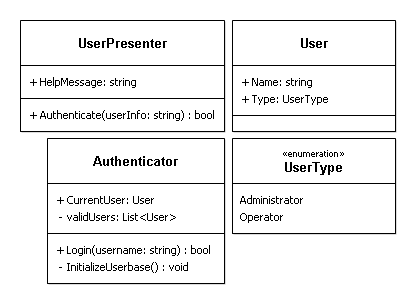
\includegraphics[scale=1]{3_2_1_authentificationsubsystem}
    \caption{Authentification Subsystem Class diagram}
    \label{fig:AuthentificationSubsystemClassDiagram}
\end{figure}

\subsubsection{Unit Descriptions}

\vspace*{0.2in}
\leftline{\textsc{UserPresenter}}
\vspace*{0.15in}
UserPresenter’s purpose is to provide information to be displayed to the LoginView; it also interfaces with the Authenticator to validate the user information submitted from the LoginView. 
\clearpage
\begin{table}[ht]
\centering
   \begin{tabular}{|l|l|}
        \hline
        {\large Name} & {\large Description} \\
        \hline\hline
        HelpMessage & Defines the messages to be displayed in the LoginView.\\
        \hline
        Authenticate & Validates the submitted string from LoginView with the\\
        & Authenticator.\\
        \hline
    \end{tabular}
\caption{UserPresenter Attributes and Methods}
\end{table}

\vspace*{0.2in}
\leftline{\textsc{Authenticator}}
\vspace*{0.15in}
Authenticator’s purpose is to log in a valid a user.  It also keeps track of the current logged in user.
\begin{table}[ht]
\centering
   \begin{tabular}{|l|l|}
        \hline
        {\large Name} & {\large Description} \\
        \hline\hline
        CurrentUser & Reference to the currently logged in user.\\
        \hline
        validUsers & List of predefined valid users to be compared against when\\
        & logging in.\\
        \hline
        Login & Sets the specified user as currently logged in, but only if it\\
        & is valid.\\
        \hline
        InitializeUserbase & Populate the list of valid users.\\
        \hline
    \end{tabular}
\caption{Authenticator Attributes and Methods}
\end{table}

\vspace*{0.2in}
\leftline{\textsc{User}}
\vspace*{0.15in}
User’s purpose is to encapsulate user information; more attributes can be added to this class as needed.
\begin{table}[ht]
\centering
   \begin{tabular}{|l|l|}
        \hline
        {\large Name} & {\large Description} \\
        \hline\hline
        Name & Specifies the name of the user as a string.\\
        \hline
        Type & Specifies the type of the user, defined by the UserType enum.\\
         & Currently, a user can either be of type Administrator or Operator.
\\
        \hline
    \end{tabular}
\caption{User Attributes and Methods}
\end{table}
\clearpage



\subsection{Simulation Subsystem}
This subsystem handles the actual logic for defining and simulating the vessels.
\subsubsection{Detailed Design Diagram}
This subsystem consists of the VesselPresenter, the Simulator, the Parser and the Vessel classes as shown in Figure~\ref{fig:SimulationSubsystemClassDiagram}.  
\begin{figure}[h!]
    \centering
    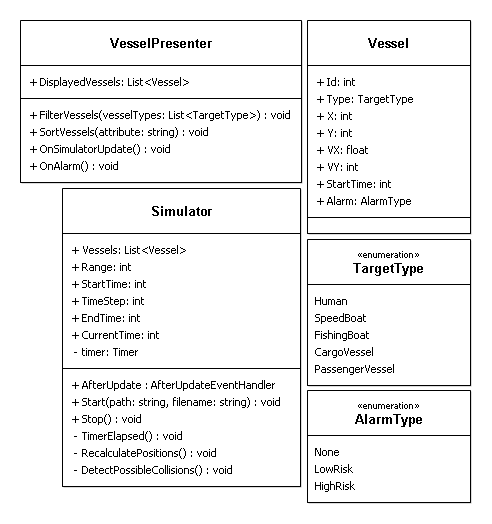
\includegraphics[scale=1]{3_3_1_simulationsubsystem}
    \caption{Simulation Subsystem Class diagram}
    \label{fig:SimulationSubsystemClassDiagram}
\end{figure}
\clearpage


\subsubsection{Unit Descriptions}
\vspace*{0.2in}
\leftline{\textsc{VesselPresenter}}
\vspace*{0.15in}
VesselPresenter’s purpose is to provide vessel information to the VesselView, RadarWidget, and the TableWidget. This includes the filtered and sorted list of vessels, as well as assuring that they are up to date information from the simulator.
\begin{table}[ht]
\centering
   \begin{tabular}{|l|l|}
        \hline
        {\large Name} & {\large Description} \\
        \hline\hline
        DisplayedVessels & List of vessels to be displayed. This is filtered and sorted; it is\\
         & the final list of vessels to be displayed by the views.\\
        \hline
        FilterVessels & Filters the vessels according to selected vessel types.\\
        \hline
        SortVessels & Sorts the vessels according to specified attribute. If the same\\
         & attribute is being sorted successively, the ordering is toggled\\
          & every time.\\
        \hline
        OnSimulationUpdate & Callback event from simulation when vessels are updated.\\
        \hline
        OnAlarm & Callback event from simulation when an alarm is generated.\\
        \hline
    \end{tabular}
\caption{VesselPresenter Attributes and Methods}
\end{table}

\vspace*{0.2in}
\leftline{\textsc{Simulator}}
\vspace*{0.15in}
Simulator’s purpose is to simulate movement for the vessels according to specified simulation properties. Regular updates are performed in order to achieve constant movement.
\clearpage
\begin{table}[ht]
\centering
   \begin{tabular}{|l|l|}
        \hline
        {\large Name} & {\large Description} \\
        \hline\hline
        Vessels & List of all active vessels to be simulated.\\
        \hline
        Range &  \\
        StartTime & Defines the properties of the simulation, as specified in the\\
        TimeStep & scenario file.\\
        EndTime & \\
        CurrentTime & \\
        \hline
        timer & A timer is used to perform updates at regular intervals. \\
        \hline
        AfterUpdate & Allow events to be registered to execute after every update.\\
        \hline
        Start & Begins simulation with the specified scenario file.\\
        \hline
        Stop & Stops the simulation.\\
        \hline
        TimerElapsed & Function called by the timer at regular intervals. Calls\\
         & RecalculatePositions and performs the AfterUpdate events.\\
        \hline
        RecalculatePositions & This is where the vessel positions are updated.\\
                             & DetectPossibleCollisions is then called. \\
        \hline
        DetectPossibleCollisions & Checks distance between vessels and generate alarms\\
                                 & if necessary.\\
        \hline
    \end{tabular}
\caption{Simulator Attributes and Methods}
\end{table}

\vspace*{0.2in}
\leftline{\textsc{Vessel}}
\vspace*{0.15in}
Vessel’s purpose is to encapsulate vessel data.
\begin{table}[ht]
\centering
   \begin{tabular}{|l|l|}
        \hline
        {\large Name} & {\large Description} \\
        \hline\hline
        Id & Id of the vessel as specified in the scenario file.\\
        \hline
        Type & Type of the vessel as specified in the scenario file. This corresponds\\
        & to a value of the TargetType enum: Human, SpeedBoat, FishingBoat,\\
        & CargoVessel, or PassengerVessel.\\
        \hline
        X & Current position coordinates of the vessel. \\
        Y &  \\
        \hline
        VX & Velocity of the vessel as specified in the scenario file.\\
        VY &  \\
        \hline
        StartTime & Time at which to start the simulation, as specified in the scenario file.\\
        \hline
        Alarm & Specifies the current alarm associated with the vessel. This\\
        & corresponds to a value from the AlarmType enum: None, LowRisk, or\\
        & HighRisk.\\
        \hline
    \end{tabular}
\caption{Vessel Attributes and Methods}
\end{table}
\clearpage

\subsection{Parsing Subsystem}
This subsystem takes care of loading initial vessel information from a scenario file.
\subsubsection{Detailed Design Diagram}
This subsystem consists of the Parser class, but also makes use of the Vessel class as shown in Figure~\ref{fig:ParsingSubsystemClassDiagram}.  
\begin{figure}[h!]
    \centering
    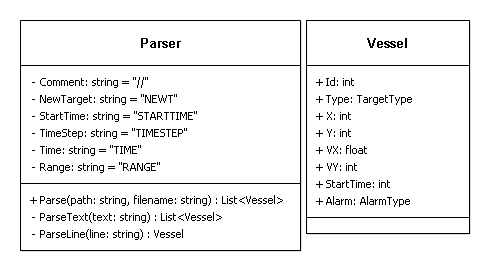
\includegraphics[scale=1]{3_4_1_parsingsubsystem}
    \caption{Parsing Subsystem Class diagram}
    \label{fig:ParsingSubsystemClassDiagram}
\end{figure}

\subsubsection{Unit Descriptions}
\vspace*{0.2in}
\leftline{\textsc{Parser}}
\vspace*{0.15in}
Parser’s purpose is to load simulation properties and initial vessel information from a scenario file.
\clearpage
\begin{table}[ht]
\centering
   \begin{tabular}{|l|l|}
        \hline
        {\large Name} & {\large Description} \\
        \hline\hline
        Comment &  \\
        NewTarget &  \\
        StartTime & Defines the keywords to look for when parsing the text file.\\
        TimeStep &  \\
        Time &  \\
        Range &  \\
        \hline
        Parse & Reads the specified scenario file and loads the list of vessels as well as\\
         & simulation properties. The actual implementation is done in ParseText\\
          & and ParseLine functions.\\
        \hline
        ParseText & Reads a block of text and separates it into lines; these lines are then\\
         & processed using ParseLine function iteratively.\\
        \hline
        ParseLine & Processes a line of text by determining which keyword matches with\\
         & the first word. The data is then stored accordingly.\\
        \hline
    \end{tabular}
\caption{Parser Attributes and Methods}
\end{table}




\clearpage
%%%%%%%%%%%%%%%%%%%%%%%%%%%%%%%%%%%%%%%%%%%%%%%%%%%%%%%%%%%%%%
%                      Part 4                       
%%%%%%%%%%%%%%%%%%%%%%%%%%%%%%%%%%%%%%%%%%%%%%%%%%%%%%%%%%%%%%


\section{Dynamic Design Scenarios}

Two main dynamic scenarios are filtering vessels and triggering risk alarms. Each is highly dynamic in nature as the states change frequently as the system is running. 

\subsection{Filtering Vessels}

Filtering is activated by the user checking or unchecking a checkbox. As we can see in Figure~\ref{fig:FilterSystemSequenceDiagram}, once a checkbox is modified, the system will remove (or add) the vessels from the list. In Figure~\ref{fig:FilterUnitSequenceDiagram}, the VesselsView asks the VesselsPresenter to return a filtered list of vessel by calling the functio GetVessel() and passing the type of vessel to filter on. The VesselsView then refreshes its list and blips based on the new list.\\

\begin{figure}[h!]
    \centering
    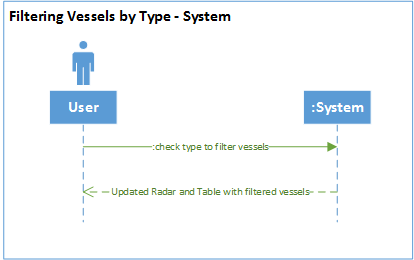
\includegraphics[scale=0.9]{4_filter_system}
    \caption{Filter System Sequence Diagram}
    \label{fig:FilterSystemSequenceDiagram}
\end{figure}

\begin{figure}[h!]
    \centering
    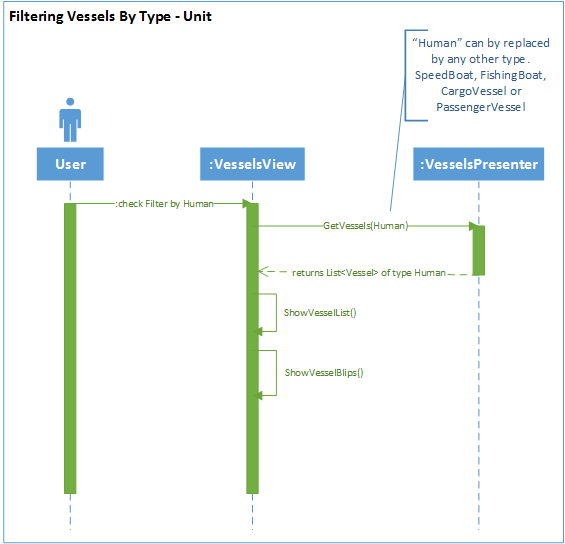
\includegraphics[scale=0.9]{4_filter_unit}
    \caption{Filter Unit Sequence Diagram}
    \label{fig:FilterUnitSequenceDiagram}
\end{figure}

\clearpage

\subsubsection{Filtering Contracts}

\begin{table}[ht]
\centering
   \begin{tabular}{|l|l|}
        \hline
        Contract Name & Filter\\
        \hline
        Use Case & Filtering Vessels by Type\\
        \hline
        Preconditions & \ - User must be an Admin.\\
                      & \ - A checkbox with the filter type must exist in the GUI.\\
                      & \ - The state of a checkbox on the GUI must be modified.\\
        \hline
        Postconditions & \ - The table is refreshed with the filtered list.\\
                       & \ - The radar is refresehd with the filtered list.\\
        \hline
    \end{tabular}
\caption{Filter Contract}
\end{table}

\clearpage

\subsection{Triggering Risk Alarms}

Triggering risk alarms is activated when at least two vessels are less than 200 meters of each other. As we can see in Figure~\ref{fig:TriggerRiskAlarmsSystemSequenceDiagram}, the VesselsPresenter subscribes to an event that is raised when a possible collision is detected. In Figure~\ref{fig:TriggerRiskAlarmsUnitSequenceDiagram}, the VesselsPresenter first subscribes to the OnAlarm event. The simulator at every time step recalculates the new position of the vessels in vessels list. It calls DetectPossibleCollisions(), and if a possible collision is found it automatically raises the OnAlarm event.

\begin{figure}[h!]
    \centering
    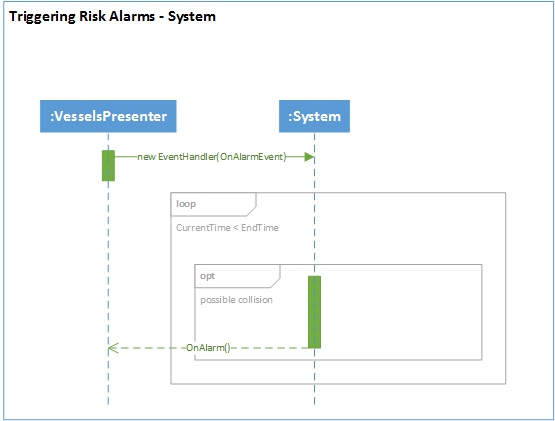
\includegraphics[scale=0.85]{4_triggering_risk_alarms_system}
    \caption{Trigger Risk Alarms System Sequence Diagram}
    \label{fig:TriggerRiskAlarmsSystemSequenceDiagram}
\end{figure}

\clearpage

\begin{figure}[h!]
    \centering
    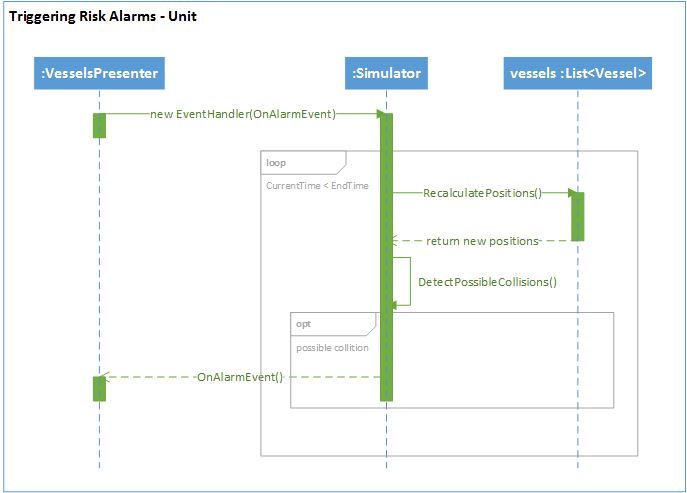
\includegraphics[scale=0.85]{4_triggering_risk_alarms_unit}    
    \caption{Trigger Risk Alarms Unit Sequence Diagram}
    \label{fig:TriggerRiskAlarmsUnitSequenceDiagram}
\end{figure}

\subsubsection{Triggering Risk Alarms Contracts}

\begin{table}[ht]
\centering
   \begin{tabular}{|l|l|}
        \hline
        Contract Name & Trigger Risk Alarms\\
        \hline
        Use Case & Triggering Risk Alarms\\
        \hline
        Preconditions & \ - Two vessels must be less than 200 meters of each other together.\\                      
        \hline
        Postconditions & \ - The OnAlarm event is raised.\\                       
        \hline
    \end{tabular}
\caption{Trigger Risk Alarms Contract}
\end{table}

\clearpage

%%%%%%%%%%%%%%%%%%%%%%%%%%%%%%%%%%%%%%%%%%%%%%%%%%%%%%%%%%%%%%
%                      Part 5                    
%%%%%%%%%%%%%%%%%%%%%%%%%%%%%%%%%%%%%%%%%%%%%%%%%%%%%%%%%%%%%%


\section{Revised Cost Estimation}
\subsection{Resources Re-evaluation}
In line with Delivery 1, some aspect of Resources allocation and planning will be discarded: Physical Resources (e.g.: Machinery, Vehicule, etc), Real Estate Resources (e.g.: Building, Rent, etc) and Financial Resources (e.g.: Financing, Budgeting, etc.) will once again be ignored. Also, Human Resources allocation is directly inherited from Delivery 1 to this document, and will not be covered again. Technical Resource allocation and consumption has not changed as well, therefore it will also be inherited from Delivery 1. One final item will not be modified from Delivery 1 is the Risk assessment. Considering that Risk requires some dedicated resources to handle or prevent it, we will assume the same risk levels and dedicated resources to it.
\\
On the other hand, the scheduling and time allocations have greatly changed from the initial scheduling in Delivery 1 to now, as the requirements for Delivery 2 and 3 have changed, and so did our methods.


\subsection{Updated Schedule}
In order to be more in line with our hybrid Agile XP/SCRUM model, we have modified our anticipated schedule for Delivery 2 and 3, as demonstrated in the following Gantt Charts in Figure~\ref{fig:JuneGanttChart}, Figure~\ref{fig:JulyGanttChart}, and Figure~\ref{fig:AugustGanttChart} respectively representing charts for the month of June, July and August.
\par
As reference, we have two Milestones left, both indicated on the chart by a blue mark, representation the due dates for Deliverable 2 (D2) and Deliverable 3 (D3). As mentioned earlier, the development time dedicated to getting the code ready to implement the GUI with the VMS together is evenly distributed between development and debugging/testing.  We allow ourselves a two day debugging buffer prior to the implementation period as well as two days of post-implementation debugging period. The implementation time has been estimated unanimously to 3 days by the programming team, which will then lead us to the actually second delivery.\par
	Considering the modifications to the requirements of Delivery 3 versus what was originally planned, the entire ensuing planning done in Delivery 1 had to be modified. And now that Delivery 3’s requirements have been disclosed, we can fully plan our next steps.\par

Extract from Delivery 1, regarding the expected requirements of each Deliveries:\newline
“According to the document ‘Project Information’, Section 1, Part 2 (Teams and Roles), each
delivery had specific goals to achieve:\newline
- \ Delivery 1: “design of the interface for the core application.”\newline
- \ Delivery 2: “creating the design.”\newline
- \ Delivery 3: “designing UI” ”\par

Extract from Delivery 3 requirements:\newline
- \ Testing \& Testing Reports\newline
- \ Testing Coverage, Items \& Cases\newline
- \ Delivery of the Functioning Systems\newline
- \ User \& Installation Manuals\newline
- \ Final Cost Revision
\par

As stipulated across the Gantt charts for the months of July and August, 100\% of the time after the handing in of Delivery 2 will be dedicated to the testing phase in accordance with the requirements of Delivery 3. Unspecified, but implied, documentation work will be done on a regular basis both during the completion of Delivery 2 as well as Delivery 3. The redaction of the User and Installation manual will start after Delivery 2 has been submitted. Considering some team members have classes other than this current course, and/or work during the day, we estimate that between 2 to 3 hours will be dedicated daily to the project by team members. 
\vspace*{0.2in}

\begin{figure}[h!]
    \centering
    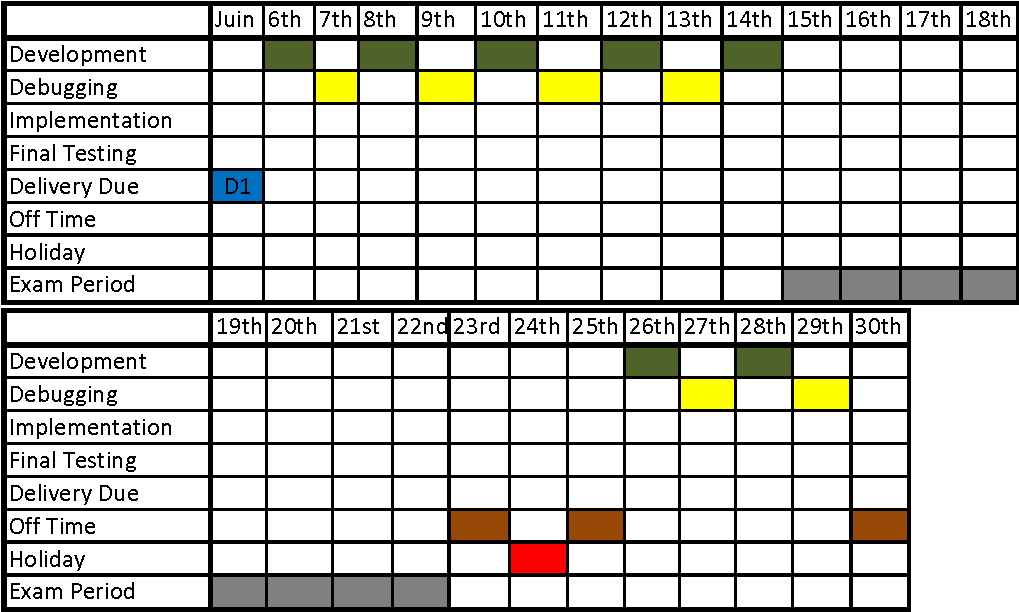
\includegraphics[scale=0.5]{Gantt_june}
    \caption{June Gantt Chart}
    \label{fig:JuneGanttChart}
\end{figure}
\begin{figure}[h!]
    \centering
    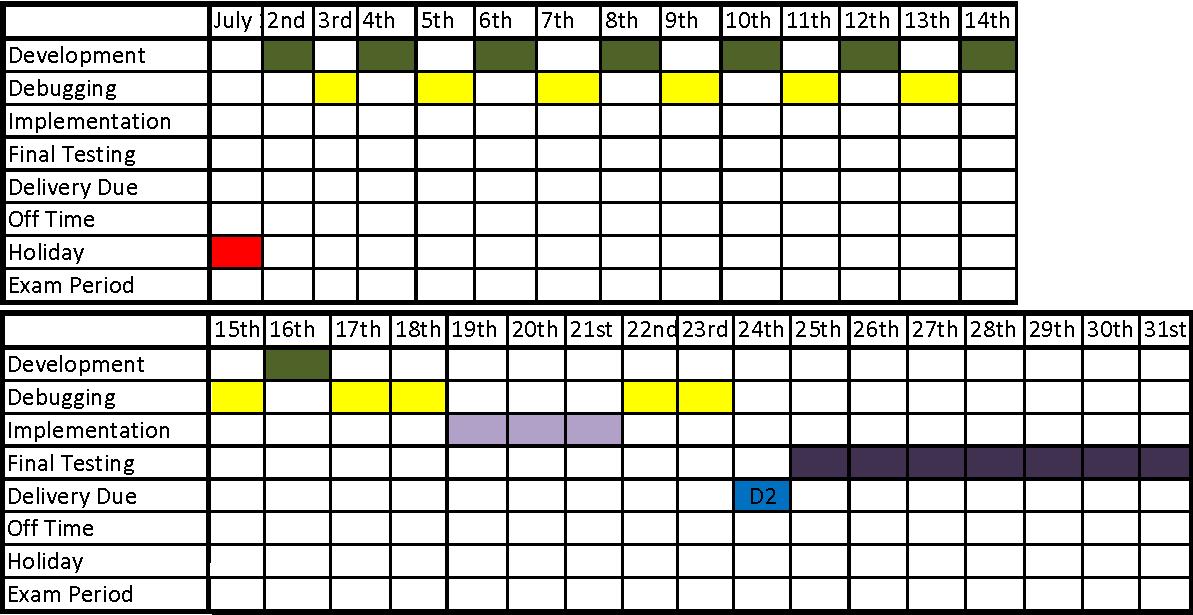
\includegraphics[scale=0.5]{Gantt_july}
    \caption{July Gantt Chart}
    \label{fig:JulyGanttChart}
\end{figure}
\begin{figure}[h!]
    \centering
    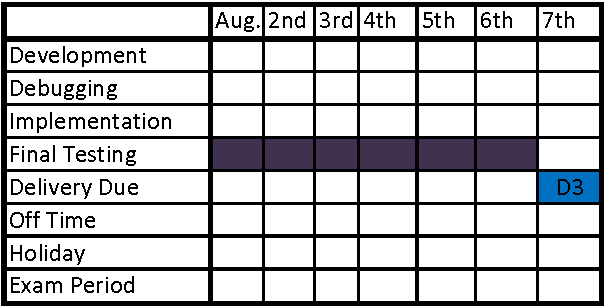
\includegraphics[scale=0.8]{Gantt_august}
    \caption{August Gantt Chart}
    \label{fig:AugustGanttChart}
\end{figure}




\end{document}